\chapter{Formal Grammars}
\label{chap:formal_grammars}
\section{Language vs Grammar}
    \theoremstyle{definition}
    \begin{definition}[Grammar]
        The (formal) definition (\textit{description}) of a language
    \end{definition}
    \theoremstyle{definition}
    \begin{definition}[Language]
        A (potentially infinite) \textit{set} of sentences, in programming language, a
        sentence is a source file, REPL expression, etc.
    \end{definition}
    \theoremstyle{definition}
    \begin{definition}[Alphabet]
        Composed of tokens, lexemes.
    \end{definition}

    Let's take an example which is JSON.  The language is all valid JSON
    expression.
    Sentences : e.g. 
    \begin{figure}[H]
         \centering
         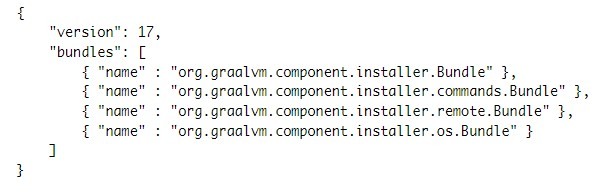
\includegraphics[scale=0.6]{JSON_sentence.jpg}
         \caption{JSON Sentence}
         \label{fig:json_sentence}
    \end{figure}
    Grammar : 
    \begin{figure}[H]
         \centering
         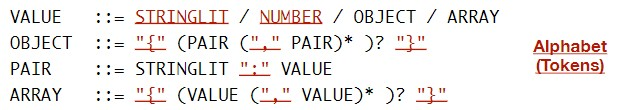
\includegraphics[scale=0.6]{JSON_Grammar.jpg}
         \caption{JSON Grammar}
         \label{fig:json_grammar}
    \end{figure}
\section{Grammar notation}
    \subsection{PEG}
        Parsing Expression Grammar. The "?" denotes optional, "*" means 0 or more
        times.
        \begin{figure}[H]
             \centering
             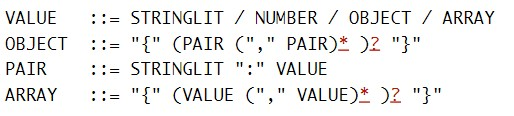
\includegraphics[scale=0.6]{PEG.jpg}
             \caption{PEG notation}
             \label{fig:label}
        \end{figure}
        PEG is a grammar formalism and a notation.
        \theoremstyle{definition}
        \begin{definition}[Formalism]
            Mathematical system to define the language (set of sentences)
        \end{definition}
        \theoremstyle{definition}
        \begin{definition}[Notation]
            A way to denote a grammar to be interpreted by the formalism.
        \end{definition}
    \subsection{EBNF and BNF}
        Note that (E)BNF is a notation for CFG (Context-Free Grammars).
        \subsubsection{EBNF}
            Extended Backus-Naur Form. "[]" means optional, "\{\}" means 1 or more
            times, so in order to make "0 or more" with have to combine symbols.
            \begin{figure}[H]
                \centering
                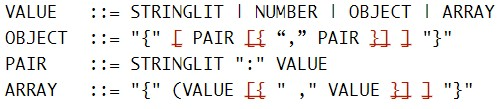
\includegraphics[scale=0.6]{EBNF.jpg}
                \caption{EBNF notation}
                \label{fig:ebnf}
            \end{figure}
        \subsubsection{BNF}
            Backus-Naur Form. It is at the base of EBNF, it does not contain "\{\}"
            or "[]", so it uses recursion and a lot more rules. Note that $\epsilon$
            is the mathematical notation for "nothing"
            \begin{figure}[H]
                \centering
                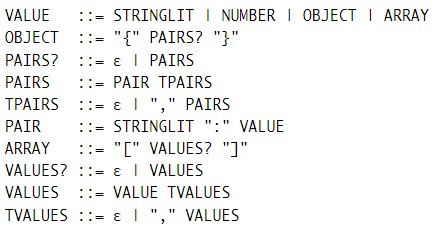
\includegraphics[scale=0.6]{BNF.jpg}
                \caption{BNF notation}
                \label{fig:bnf}
            \end{figure}
    \subsection{Summary}
        CFG and PEG are different formalism. In some case, PEG and CFG can be
        the same (like in JSON) because it is a very simple definition. By it is
        not true in general. Sometimes, we can use PEG notations like +, *, ? in
        CFGs (coming from REGEx, which are related to CFGs.). Actually we can
        use any notation that we want, we just need to define it!